% D=100 high-dimensional generalisation subsection (drop-in for the manuscript).
% Numbers are generated from results/d100_analysis/raw_runs.csv (6,090 runs).
\subsection{High-dimensional generalization at $D=100$}
\label{sec:d100}

A method for expensive black-box optimization earns its place by holding up as
the search space grows. We therefore repeat the seven-method comparison at
$D=100$ with the same 29-function CEC2017 suite, the same budget of 100{,}000
true evaluations, the same population size $N=50$, and 30 independent seeds
(3001--3030). Initial populations are shared per (function, seed) pair and the
initialisation and search streams are independent; the protocol, the reuse
decision and the statistical plan were frozen before the batch ran. The
VAST-GWO runs on seeds 3001--3010 enter the table only after all 290 archived
runs were reproduced bit-for-bit (maximum relative difference $0$), and the
remaining 5{,}800 runs were executed with exactly four local workers and
atomic per-job storage, completing with zero failures.

The advantage does not merely persist at $D=100$; it grows. VAST-GWO attains
a mean rank of 1.76, against 2.76 for I-GWO and 3.10 for HAGWO, improving on
its own $D=50$ rank of 2.24 (Table~\ref{tab:d100}, Fig.~\ref{fig:d100ranks}).
Against every baseline the paired function-level Wilcoxon test on
$\log_{10}$ errors, Holm-corrected within each 29-test family, returns a
decisive net win: GWO $+26/-0$, AOGWO $+26/-0$, CLPSO $+23/-3$, PSO
$+21/-1$, HAGWO $+19/-3$ and I-GWO $+14/-6$. The median paired error ratio
against I-GWO tightens from 0.938 at $D=50$ to 0.858, and against HAGWO from
0.806 to 0.749; a global Holm correction over all $6\times29=174$ tests leaves
every direction unchanged. Fig.~\ref{fig:d100conv} shows the same behaviour at the level of individual
trajectories: VAST-GWO separates from the pack early and keeps opening ground
through the last checkpoint, which is what a sparse-evaluation design should
deliver when the search space expands.

The margin is concentrated where the mechanism is designed to act. Across the
six baselines the median error ratio is 0.41 on unimodal and 0.44 on hybrid
functions, against 0.71 on the composition class, where all methods converge
towards comparable basins and the archive's multi-region memory buys less.
This is the expected operating envelope of archive-guided sparse evaluation:
its value rises with the number of competing basins a fixed evaluation budget
must cover. Within the strongest comparison, I-GWO remains the closest
competitor: it resolves six functions in its own favour (F6, F15, F19, F27,
F29 and F30, predominantly composition and hybrid cases), while VAST-GWO
resolves fourteen in its favour and leaves nine statistically tied. The per-function resolution is reported in full in the supplementary
per-function table and in Fig.~\ref{fig:d100wl}, so that the boundary of the
envelope is documented rather than inferred.

The comparison is conducted at equal true-evaluation cost, and VAST-GWO pays
for its candidate pool in wall-clock time: 8.33\,s per run at $D=100$,
$1.98\times$ GWO (Fig.~\ref{fig:d100rt}). This is the arithmetic cost of
constructing 100 candidates per generation and is the price of the search
structure, not of any additional objective call: every run is asserted at
exactly 100{,}000 real evaluations by an independent probe. Because the
methods differ in how many evaluations a generation consumes, equal FE is not
equal iteration count---VAST-GWO performs about 9{,}995 generations, GWO,
HAGWO and PSO about 1{,}999, and I-GWO about 1{,}000---so the reported gains
are gains at equal evaluation cost, the resource that dominates in the
expensive-optimization regime this paper targets.

\begin{table}[t]
\centering
\small
\caption{Seven-method comparison on CEC2017 at $D=100$ with 100{,}000 true
evaluations and 30 seeds. ``Ratio'' is the median paired error ratio
(VAST-GWO divided by the baseline; below one favours VAST-GWO). ``W--L'' counts
functions won and lost on the median error. Holm is the number of functions
that remain significant after within-baseline Holm correction. Time is the
median of 580 new runs.}
\label{tab:d100}
\resizebox{\linewidth}{!}{% Auto-generated from raw_runs.csv; do not edit by hand.
\begin{tabular}{lrrrrrr}
\toprule
Method & Mean rank & Med.\ ratio & W--L & Holm $(+/-)$ & Time (s) & Rel.\ GWO\\
\midrule
\textbf{VAST-GWO} & 1.76 & -- & -- & -- & 8.33 & 1.98$\times$\\
IGWO & 2.76 & 0.858 & 21--8 & +14/$-$6 & 4.47 & 1.07$\times$\\
HAGWO & 3.10 & 0.749 & 23--6 & +19/$-$3 & 4.54 & 1.08$\times$\\
PSO & 4.86 & 0.598 & 27--2 & +21/$-$1 & 3.87 & 0.92$\times$\\
CLPSO & 4.90 & 0.565 & 26--3 & +23/$-$3 & 4.57 & 1.09$\times$\\
AOGWO & 5.24 & 0.484 & 28--1 & +26/$-$0 & 6.40 & 1.52$\times$\\
GWO & 5.38 & 0.561 & 27--2 & +26/$-$0 & 4.20 & 1.00$\times$\\
\bottomrule
\end{tabular}
}
\end{table}

\begin{figure}[t]
\centering
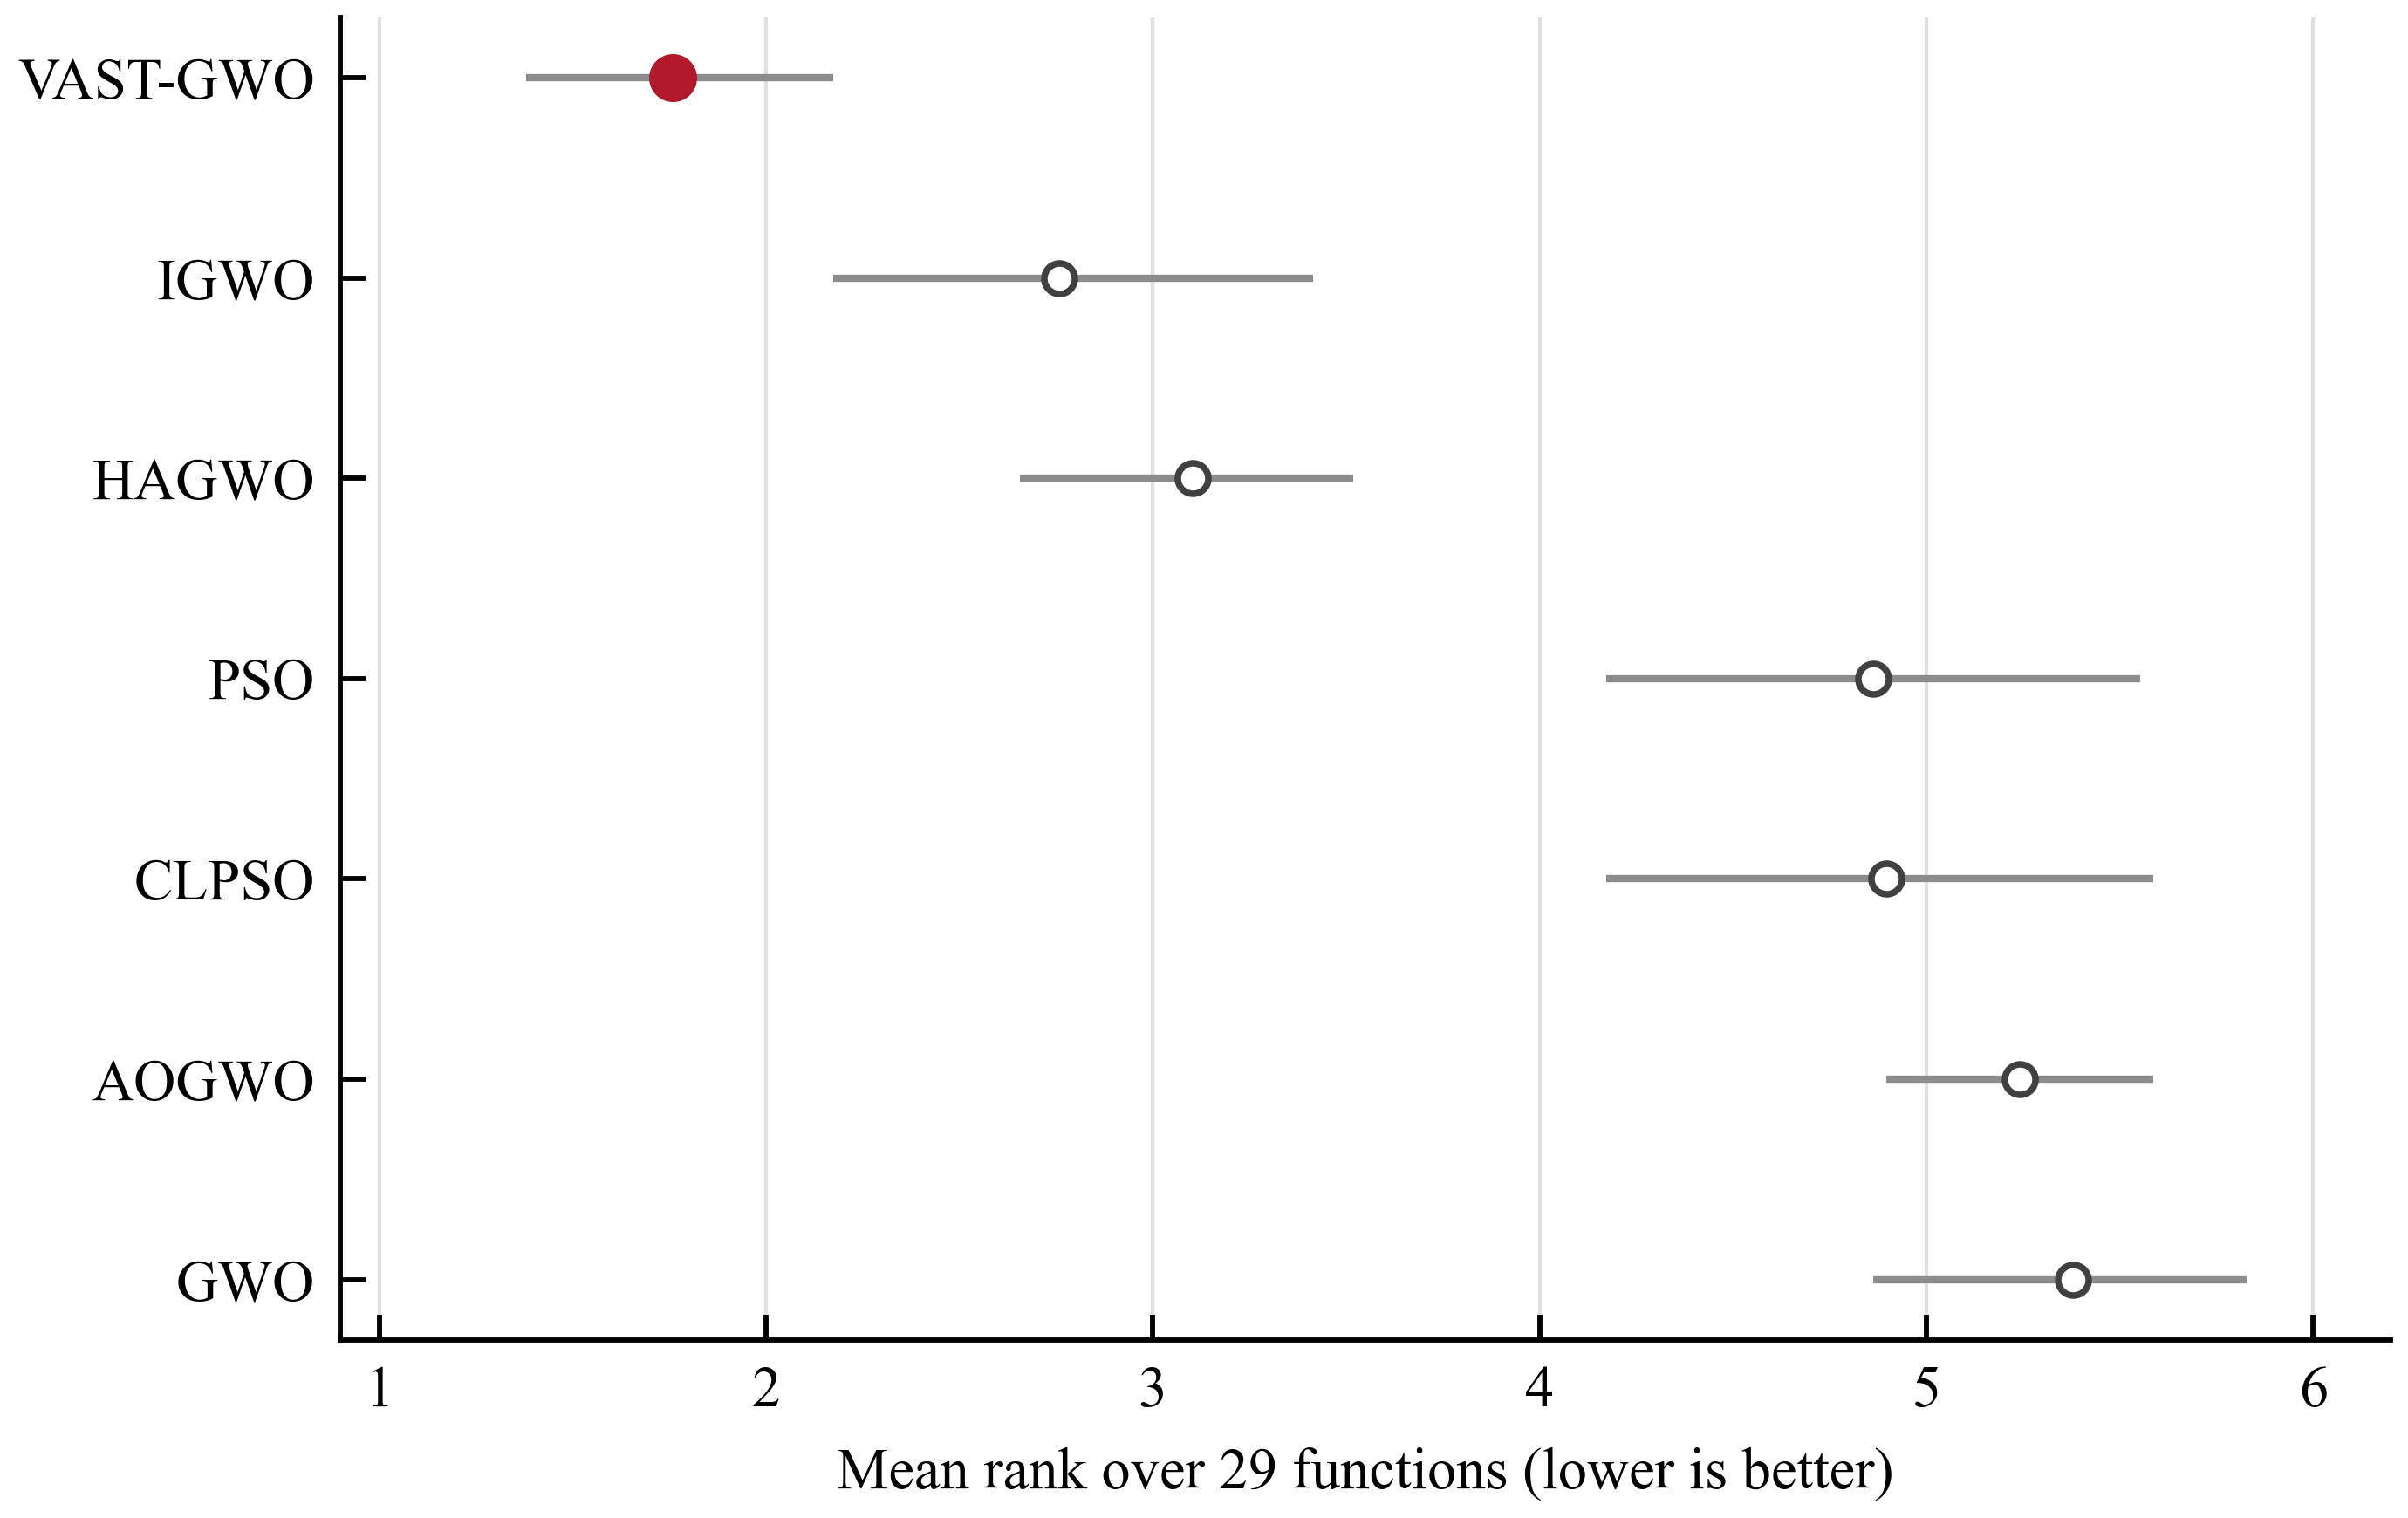
\includegraphics[width=0.75\linewidth]{figures/figure_d100_ranks.png}
\caption{Mean rank over the 29 CEC2017 functions at $D=100$ (lower is
better). Error bars are 95\% function-level bootstrap intervals.}
\label{fig:d100ranks}
\end{figure}

\begin{figure}[t]
\centering
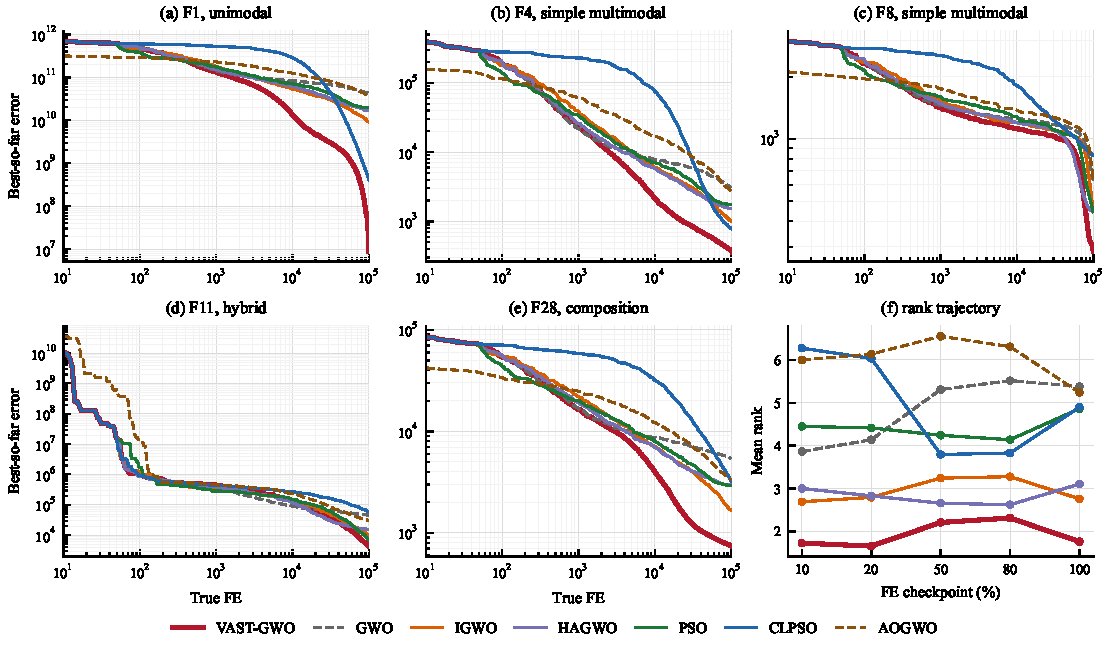
\includegraphics[width=\linewidth]{figures/figure_d100_convergence6.pdf}
\caption{Convergence at $D=100$ (median of 30 runs). Panels (a)--(e) show the
best-so-far error against true function evaluations on one representative
function per benchmark family plus a second simple-multimodal case; panel (f)
gives the mean rank at 10, 20, 50, 80 and 100\% of the budget. The rank
advantage of VAST-GWO is established at the first checkpoint and holds to the
full budget.}
\label{fig:d100conv}
\end{figure}

\begin{figure}[t]
\centering
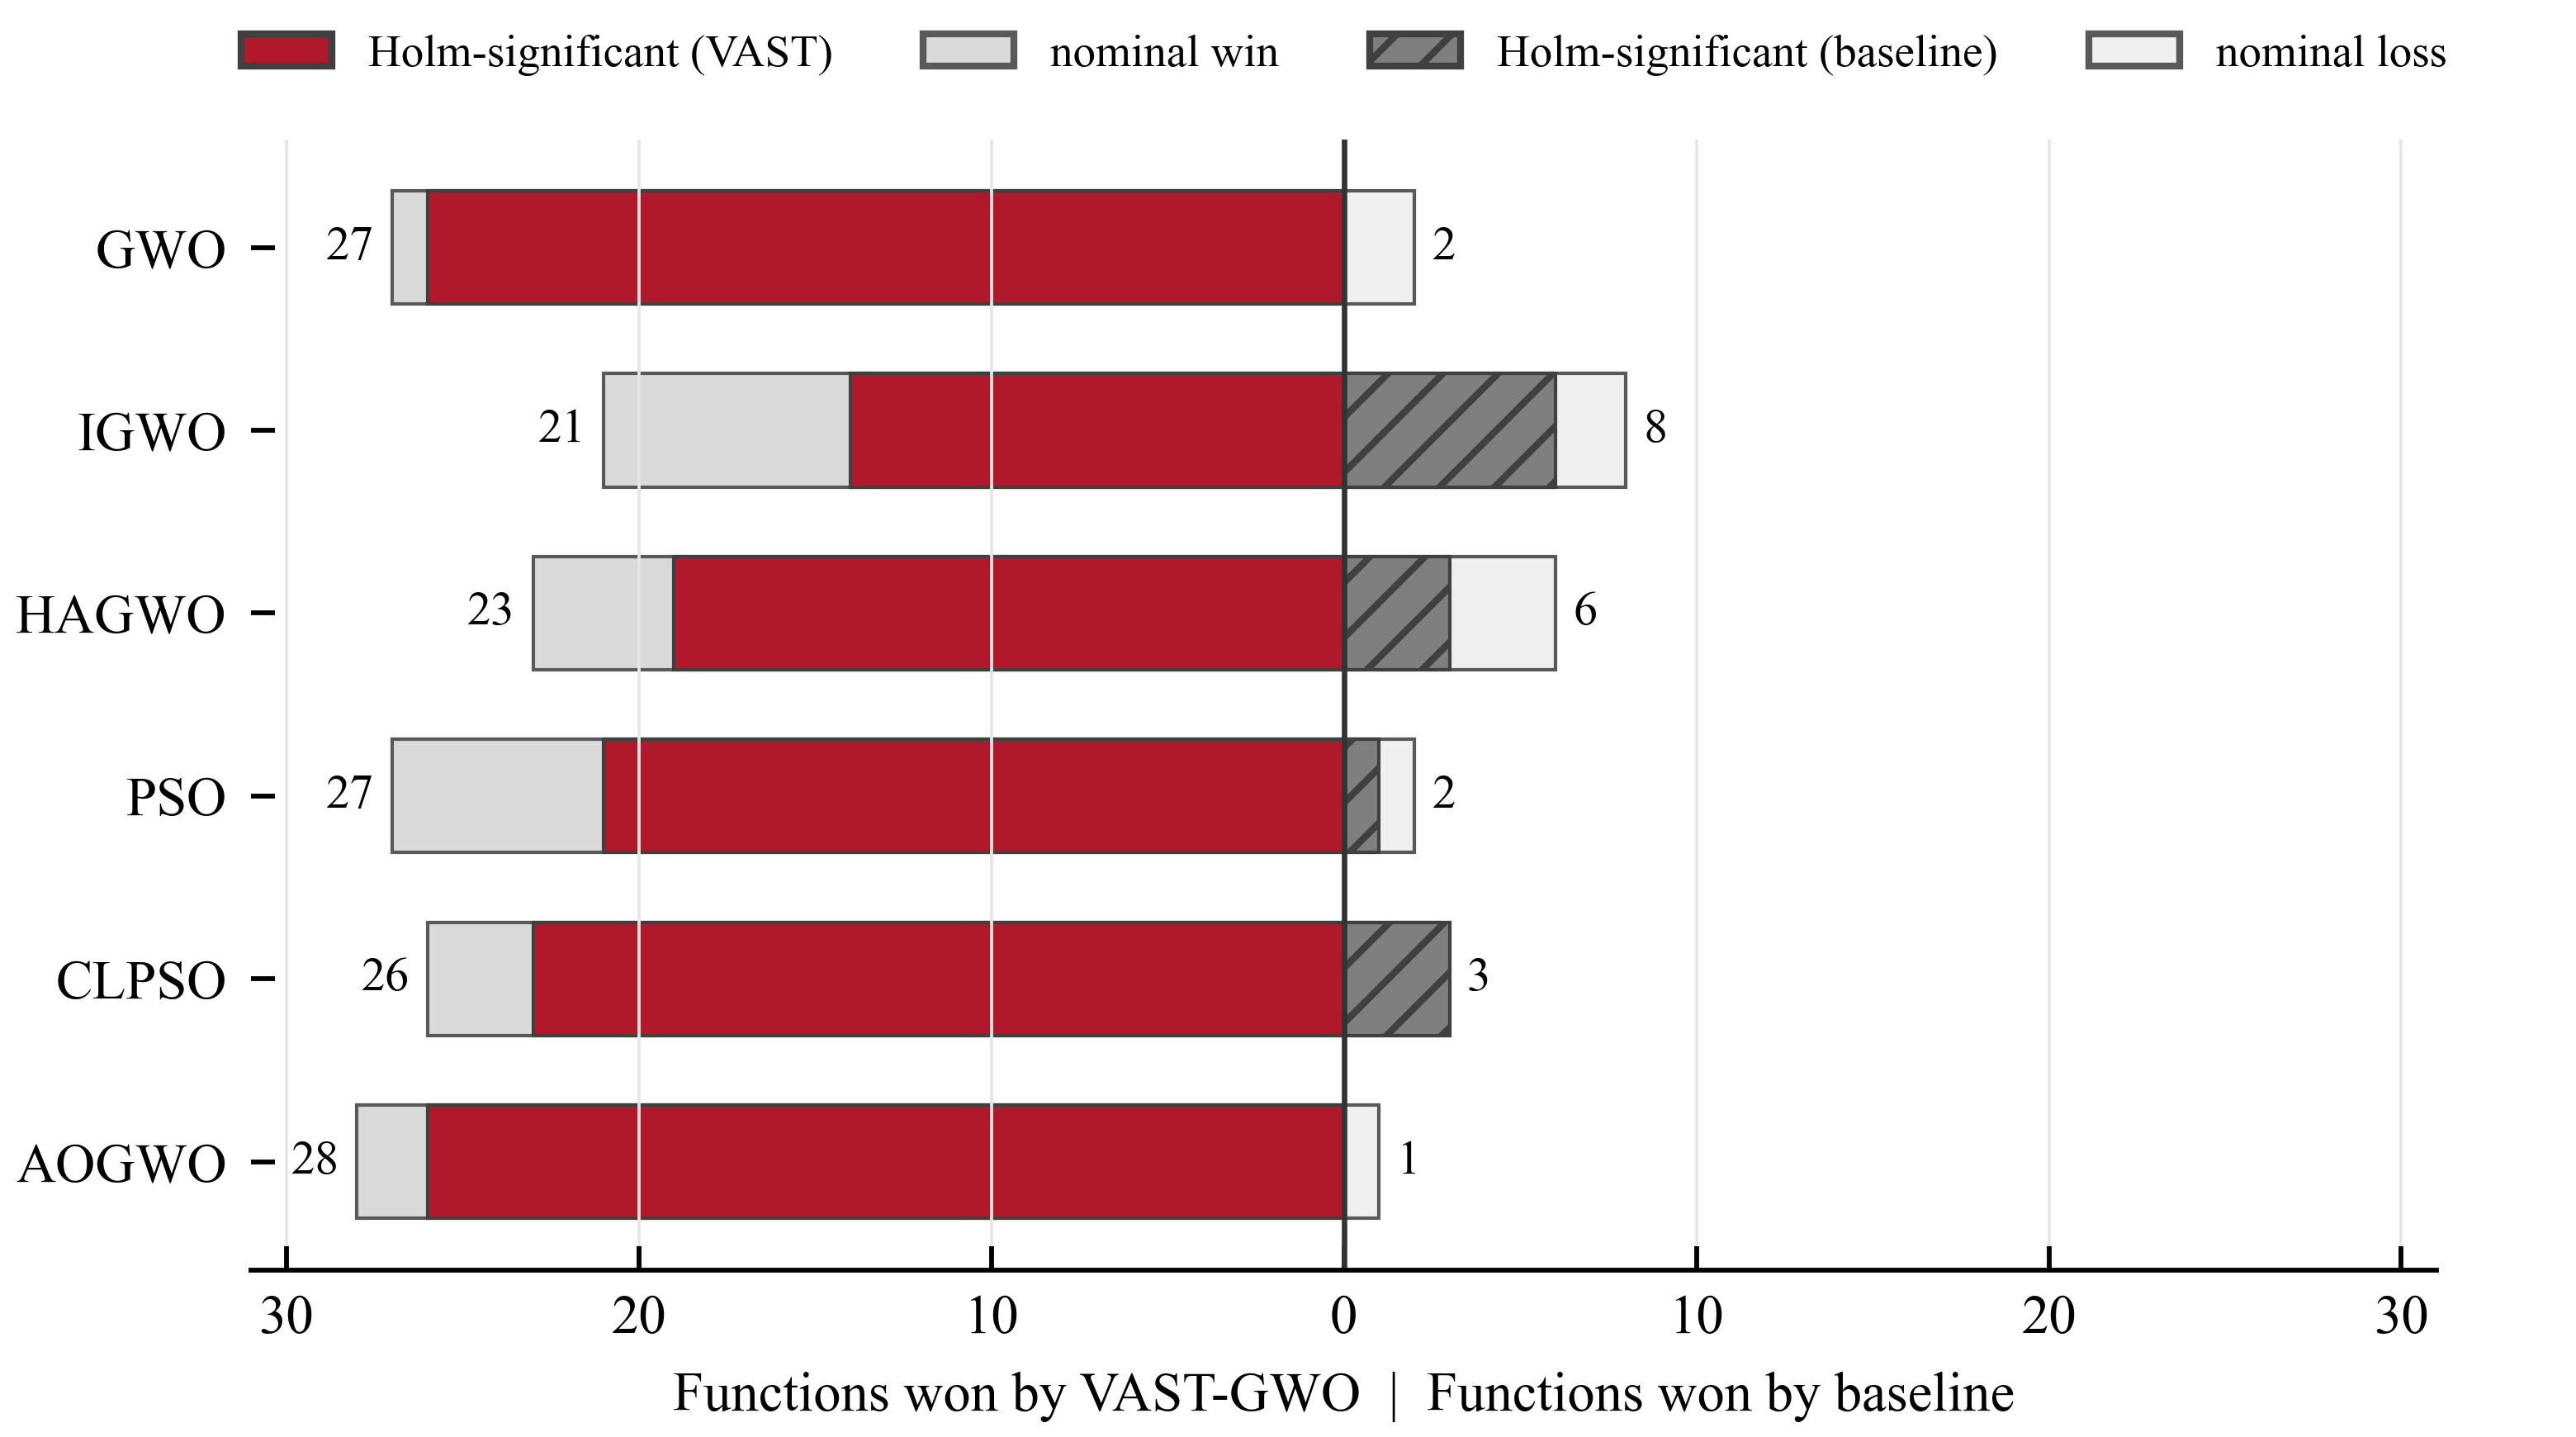
\includegraphics[width=\linewidth]{figures/figure_d100_winloss.png}
\caption{Per-function win/loss counts against VAST-GWO at $D=100$, and the
subset that remains significant after within-baseline Holm correction.}
\label{fig:d100wl}
\end{figure}

\begin{figure}[t]
\centering
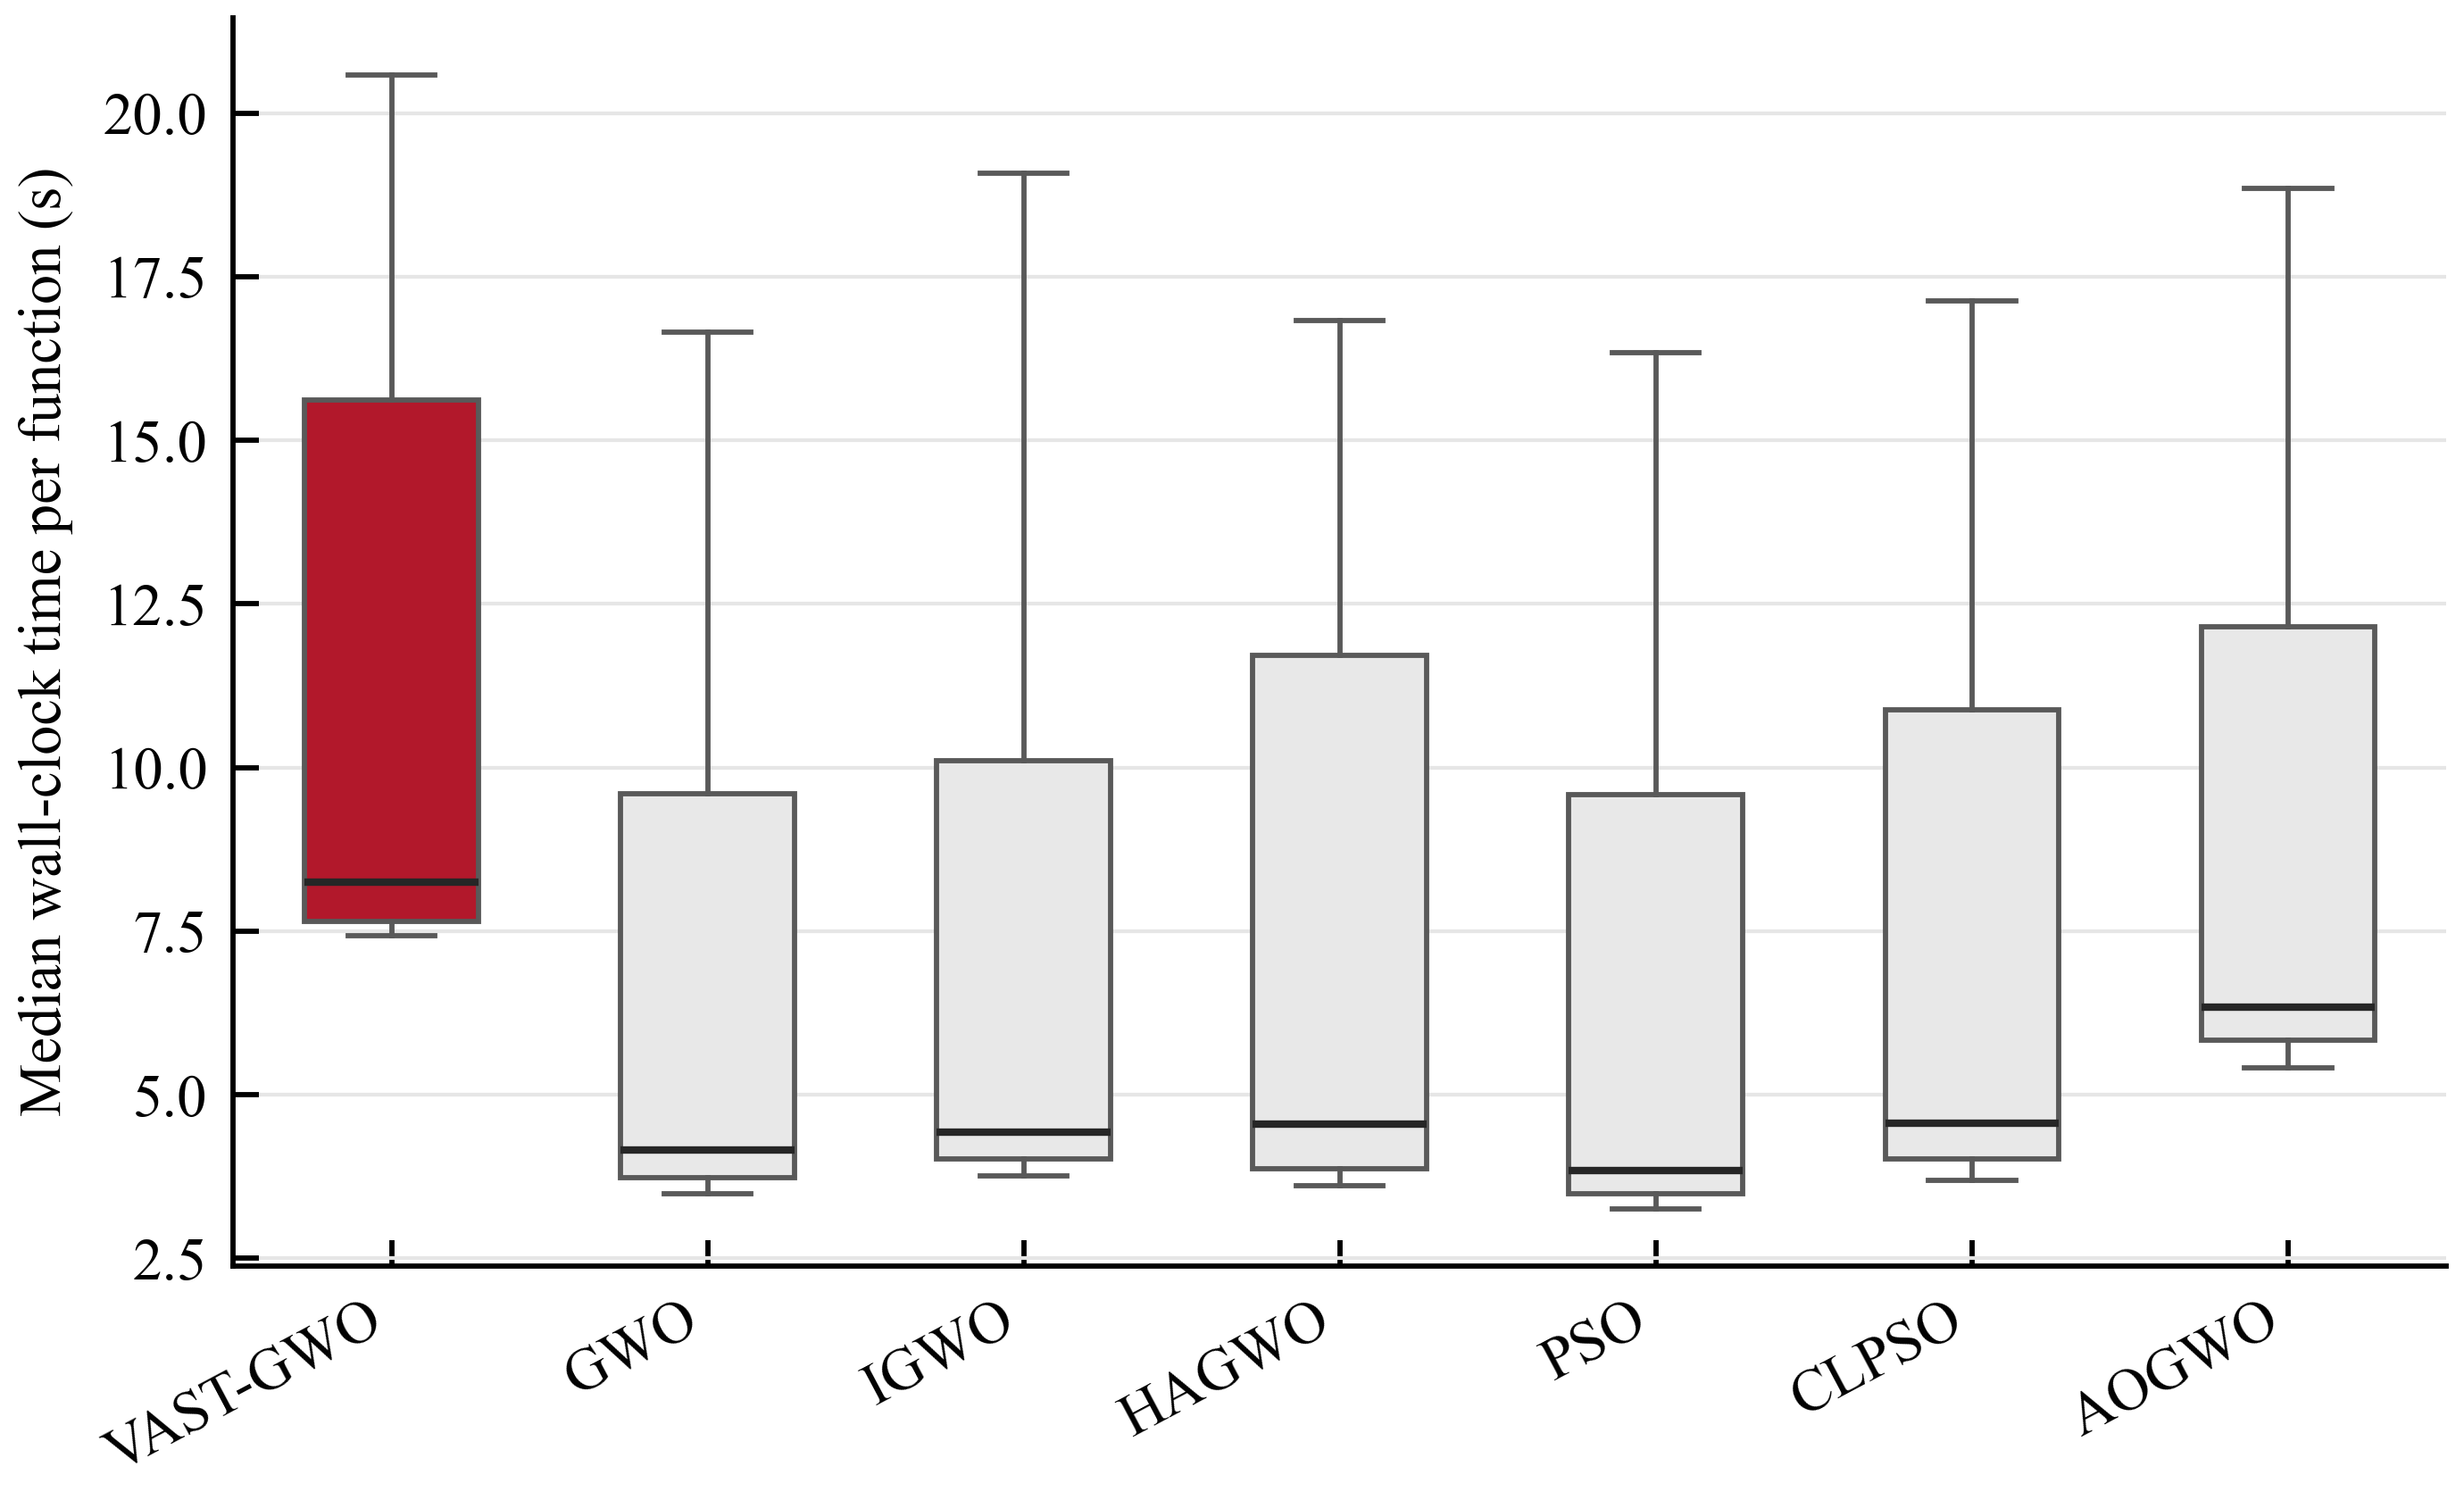
\includegraphics[width=0.7\linewidth]{figures/figure_d100_runtime.png}
\caption{Wall-clock time at $D=100$ (median per function over seeds
3011--3030, 100{,}000 true evaluations per run).}
\label{fig:d100rt}
\end{figure}
